% rasti_template.tex 
%
% LaTeX template for creating an RASTI paper
%
% v1.0 released 12 November 2021
% (version numbers match those of rasti.cls)
%
% Copyright (C) Royal Astronomical Society 2021
% Authors:
% Peter Jones (OUP, adapted from mnras_template.tex, author Keith T. Smith (Royal Astronomical Society))

% Change log
%
% v1.0 November 2021
%    Adapted from mnras_template.tex


%%%%%%%%%%%%%%%%%%%%%%%%%%%%%%%%%%%%%%%%%%%%%%%%%%
% Basic setup. Most papers should leave these options alone.
\documentclass[fleqn,usenatbib]{rasti}

% RASTI is set in Times font. If you don't have this installed (most LaTeX
% installations will be fine) or prefer the old Computer Modern fonts, comment
% out the following line
\usepackage{newtxtext,newtxmath}
% Depending on your LaTeX fonts installation, you might get better results with one of these:
%\usepackage{mathptmx}
%\usepackage{txfonts}

% Use vector fonts, so it zooms properly in on-screen viewing software
% Don't change these lines unless you know what you are doing
\usepackage[T1]{fontenc}

% Allow "Thomas van Noord" and "Simon de Laguarde" and alike to be sorted by "N" and "L" etc. in the bibliography.
% Write the name in the bibliography as "\VAN{Noord}{Van}{van} Noord, Thomas"
\DeclareRobustCommand{\VAN}[3]{#2}
\let\VANthebibliography\thebibliography
\def\thebibliography{\DeclareRobustCommand{\VAN}[3]{##3}\VANthebibliography}


%%%%% AUTHORS - PLACE YOUR OWN PACKAGES HERE %%%%%

% Only include extra packages if you really need them. Common packages are:
\usepackage{graphicx}	% Including figure files
\usepackage{amsmath}	% Advanced maths commands
%% \usepackage{amssymb}	% Extra maths symbols
\usepackage{aas_macros}

%%%%%%%%%%%%%%%%%%%%%%%%%%%%%%%%%%%%%%%%%%%%%%%%%%

%%%%% AUTHORS - PLACE YOUR OWN COMMANDS HERE %%%%%

% Please keep new commands to a minimum, and use \newcommand not \def to avoid
% overwriting existing commands. Example:
%\newcommand{\pcm}{\,cm$^{-2}$}	% per cm-squared
\newcommand{\msun}{\mathcal{M}_{\sun}}

%%%%%%%%%%%%%%%%%%%%%%%%%%%%%%%%%%%%%%%%%%%%%%%%%%

%%%%%%%%%%%%%%%%%%% TITLE PAGE %%%%%%%%%%%%%%%%%%%

% Title of the paper, and the short title which is used in the headers.
% Keep the title short and informative.
\title[WD Photometric Toolkit]{WDPhotTools -- A White Dwarf Photometric Toolkit in Python}

% The list of authors, and the short list which is used in the headers.
% If you need two or more lines of authors, add an extra line using \newauthor
\author[M. C. Lam et al.]{
Marco C. Lam,$^{1}$\thanks{E-mail: lam@tau.ac.il}
A. N. Other,$^{2}$
and another Author$^{3}$
\\
% List of institutions
$^{1}$School of Physics and Astronomy, Tel Aviv University, Tel Aviv, Israel 69978
}

% These dates will be filled out by the publisher
\date{Accepted XXX. Received YYY; in original form ZZZ}

% Enter the current year, for the copyright statements etc.
\pubyear{2022}

% Don't change these lines
\begin{document}
\label{firstpage}
\pagerange{\pageref{firstpage}--\pageref{lastpage}}
\maketitle

% Abstract of the paper
\begin{abstract}
%%%%%%%%%%%%%%%%%%%%%%%%%%%%%%%%%%%%%%%%%%%%%%%%%%%%%%%%%%%%%%%%%%%%%%%%%%%%%%%%
From data collection to generating a white dwarf luminosity function, it
requires numerous Astrophysical, Mathematical and programming domain
knowledge. The steep learning curve makes it difficult to enter the field and
often individuals have to reinvent the wheel to perform identical data reduction
and analysis tasks. We have gathered all the publicly available white dwarf
cooling models and synthetic photometry to provide a toolkit that allows
visualisation of various models, photometric fitting of white dwarf with or
without parallax and reddening, and the computing of white dwarf luminosity
functions with a choice of initial mass function, star formation history,
initial-final mass relation, and white dwarf cooling models.

\end{abstract}

% Select between one and six entries from the list of approved keywords.
% Don't make up new ones.
\begin{keywords}
keyword1 -- keyword2 -- keyword3
\end{keywords}

%%%%%%%%%%%%%%%%%%%%%%%%%%%%%%%%%%%%%%%%%%%%%%%%%%
%%%%%%%%%%%%%%%%% BODY OF PAPER %%%%%%%%%%%%%%%%%%

\section{Introduction}
%%%%%%%%%%%%%%%%%%%%%%%%%%%%%%%%%%%%%%%%%%%%%%%%%%%%%%%%%%%%%%%%%%%%%%%%%%%%%%%%
White dwarfs~(WDs) are the final stage of stellar evolution of main
sequence~(MS) stars with zero age MS~(ZAMS) mass less than $8\msun$. Since this
mass range encompasses the vast majority of stars in the Galaxy, these
degenerate remnants are the most common final product of stellar evolution,
thus providing a good sample to study the history of stellar evolution and star
formation in the Galaxy. In this state, there is little nuclear burning to
replenish the energy they radiate away. As a consequence, the luminosity and
temperature decrease monotonically with time. The electron degenerate nature
means that a WD with a typical mass of $0.6\mathcal{M}_{\sun}$ has a similar
size to the Earth, giving rise to their high densities, low luminosities, and
large surface gravities.

%%%%%%%%%%%%%%%%%%%%%%%%%%%%%%%%%%%%%%%%%%%%%%%%%%%%%%%%%%%%%%%%%%%%%%%%%%%%%%%%
The use of the white dwarf luminosity function~(WDLF) as cosmochronometer was
first introduced by \citet{1959ApJ...129..243S}. Given a finite age of the
Galaxy, there is a minimum temperature below which no white dwarfs can reach in
a limited cooling time. This limit translates to an abrupt downturn in the WDLF
at faint magnitudes. Evidence of such behaviour was observed by
\citet{1979ApJ...233..226L}, however, it was not clear at the time whether it
was due to incompleteness in the observations or to some defect in the
theory~(e.g.,~\citealp{1984ApJ...282..615I}). A decade later,
\citet{1987ApJ...315L..77W} gathered concrete evidence for the downturn and
estimated the age\footnote{``Age'' refers to the total time since the oldest
WD progenitor arrived at the zero-age main sequence.} of the disc to be
$9.3 \pm 2.0$\,Gyr~(see also \citealt{1988ApJ...332..891L}). While most studies
focused on the Galactic discs~\citep{1989LNP...328...15L, 1992ApJ...386..539W,
1995LNP...443...24O, 1998ApJ...497..294L, 1999MNRAS.306..736K,
2012ApJS..199...29G}, some worked with the stellar
halo~\citep{2006AJ....131..571H, 2011MNRAS.417...93R, 2017AJ....153...10M,
2019MNRAS.482..715L}. 
 
%%%%%%%%%%%%%%%%%%%%%%%%%%%%%%%%%%%%%%%%%%%%%%%%%%%%%%%%%%%%%%%%%%%%%%%%%%%%%%%%
Most WDs have similar broadband colour to main sequence stars, they cannot be
identified using photometry alone. They are found from UV-excess, large
proper motion and/or parallax. Because of the strongly peaked surface gravity
distribution of WDs, photometric fitting for their intrinsic properties
is possible by assuming a surface gravity. WDs fitted in such way are useful
statistically provided that the sample is not strongly biased. This is
demonstrated in various studies comparing photometric and spectroscopic
solutions to calibrate atmosphere
model~\citep{2019ApJ...871..169G, 2019ApJ...882..106G}, as well as from the
agreeing shapes of the WDLFs from spectroscopic and photometric samples. The
Gaia satellite provides parallactic measurement for over a billion point
sources~\citep{2021A&A...649A...1G, 2021AJ....161..147B} of which $359,000$
are high confidence WD candidates~\citep{2021MNRAS.508.3877G}. The availability
of parallaxes allow much more accurate fitting, particularly without knowing
the surface gravity for the photometric sample. This has completely 
revolutionarized the field of WD sciences. In the forthcoming decade, the
Simonyi Survey Telescope at the Vera C. Rubin Observatory will continue to
discover more WDs at fainter magnitudes, but only accompanied with proper
motion measurement at best. Furthermore, at those magnitudes, it is infeasible
to collect spectrum for most of them and thus studies will mostly rely on
photometric methods.

%%%%%%%%%%%%%%%%%%%%%%%%%%%%%%%%%%%%%%%%%%%%%%%%%%%%%%%%%%%%%%%%%%%%%%%%%%%%%%%%
In this generation of user-side Astronomy data handling and analysis, as well
as in the computing courses for scientists, \texttt{Python} is among the most
popular languages due to its ease to use with a relatively shallow learning
curve, readable syntax and simple way to "glue" different pieces of software
together. Its flexibility to serve as a scripting and an object-oriented
language makes it useful in many use cases: demonstrating with visual tools
with little overhead, prototyping, web-serving, and it can be compiled if
wanted. This broad range of functionality and high-level usage make it
relatively inefficient. However, Python is an excellent choice of language to
build wrappers over highly efficient and well-established codes. In fact,
some of the most used packages, scipy~\citep{2020NatMe..17..261V} and
numpy~\citep{2020Natur.585..357H}, are written in Fortran and C respectively.
\texttt{WDPhotTools} depends heavily on these two highly optimised and matured
packages to deliver the desired efficiency.

%%%%%%%%%%%%%%%%%%%%%%%%%%%%%%%%%%%%%%%%%%%%%%%%%%%%%%%%%%%%%%%%%%%%%%%%%%%%%%%%
In this paper, it is organised as follow: in Section \textsection2, we describe
the software structure and development process. Section \textsection3 describe
the model formatter. Section \textsection4 covers the photometric fitting
procedures and the overview of the model used. It also explains the
construction of a theoretical luminosity function including some descriptions
of the models available. Section \textsection5 goes through the other tools
that are essential to the software. We conclude this work in Section
\textsection6.

%%%%%%%%%%%%%%%%%%%%%%%%%%%%%%%%%%%%%%%%%%%%%%%%%%%%%%%%%%%%%%%%%%%%%%%%%%%%%%%%
Throughout this work, we use $m$ to denote apparent magnitude, $M$ for
absolute magnitude, curly $\mathcal{M}$ to denote mass, where $\mathcal{M}_i$
for the (initial) zero-age main sequence mass, and $\mathcal{M}_f$ for the
(final) white dwarf mass.

\section{Software and Development Organisation}
%%%%%%%%%%%%%%%%%%%%%%%%%%%%%%%%%%%%%%%%%%%%%%%%%%%%%%%%%%%%%%%%%%%%%%%%%%%%%%%%
The goal for this work is to ease researchers the effort in reinventing the
wheel for trivial, repetitive but essential tasks in many aspect of data
analysis for WD science. This also allow simpler setup to compare results as a
result of the choice of models. There is already a spectroscopic version
for a similar purpose, the \textsc{wdtools}
\footnote{\url{https://github.com/vedantchandra/wdtools}}~
\citep{2020MNRAS.497.2688C}.

\textsc{WDPhotTools} can generate colour-colour diagram, colour-magnitude
diagram in various photometric systems, plotting cooling profiles from
different models, and compute theoretical white dwarf luminosity functions
based on the built-in or supplied models. The core parts of this work are
three-fold: (1)~the foundation of this work is the tailored-formatters that
handle the output models from various works in the format as they were
generated and downloaded. This allows the software to be updated to handle
future releases of the models easily; (2)~photometric fitter that solves for
the WD parameters based on the photometry, with or without distance and
reddening; and (3) to generate white dwarf luminosity function in
bolometric magnitudes or in any of the photometric systems available from the
atmosphere models.

We host our source code on Github\footnote{\url{https://github.com/cylammarco/WDPhotTools}},
which provides version control and other utilities to facilitate the
development. It offers issue and bug tracking, high-level project management,
automation with Github Actions upon each commit for:

\begin{enumerate}
    \item Continuous Integration (CI) to install the software in Linux, Mac
    and Windows system, and then perform unit tests with \textsc{pytest}
    (Krekel et al. 2004);
    \item generating test coverage report with Coveralls\footnote{\url{
    https://coveralls.io/github/cylammarco/WDPhotTools}}
    which identifies
    lines in the script that are missed from the tests;
    \item Continuous Deployment (CD) through \textsc{PyPI} that allows
    immediate availability of the latest software release; and
    \item generating application programming interface~(API) documentation
    powered by \textsc{Sphinx} hosted on
    Read the Docs\footnote{\url{https://wdphottools.readthedocs.io}}.
\end{enumerate}

% 
%@misc{pytestx.y,
%  title =        {pytest x.y},
%  author = {Krekel, Holger and Oliveira, Bruno and Pfannschmidt, Ronny and Bruynooghe, Floris and Laugher, Brianna and Bruhin, Florian},
%  year =         {2004},
%  url = {https://github.com/pytest-dev/pytest},
%}
The following is not serving as an API, it is only describing some of the key
arguments and parameters, as well as the usage that may seem convoluted but
necessary to keep the structure simple without providing multiple methods to
perform similar tasks with small adjustments. The model readers are designed
to read the files as they are downloaded from the source, such that the future
updates of the models provided by the same research group should be a
straightforward process in extending the model list. The materials that have
gone into the classes and modules are described first, and towards the end of
each of \textsection3 to \textsection6, the usage of those classes and modules
are explained.

\section{Formatters}
%%%%%%%%%%%%%%%%%%%%%%%%%%%%%%%%%%%%%%%%%%%%%%%%%%%%%%%%%%%%%%%%%%%%%%%%%%%%%%%%
There are two classes of model readers, one is for reading the synthetic
photometry computed from the Montreal DA/DB atmosphere models; the other one is
a formatter that handled the different formats in the output files from
different providers.

\subsection*{Synthetic Photometry}
%%%%%%%%%%%%%%%%%%%%%%%%%%%%%%%%%%%%%%%%%%%%%%%%%%%%%%%%%%%%%%%%%%%%%%%%%%%%%%%%
The only synthetic photometry publicly available over a smooth grid of wide
ranges of temperature and surface gravity is the Montreal
model\footnote{\url{https://www.astro.umontreal.ca/~bergeron/CoolingModels/}}.
The tables are provided with bolometric and absolute magnitudes on various
photometric systems in pure hydrogen~(DA) and pure-helium~(DB) in the range of
$\log(g)=7.0 - 9.0$, as well as the effective temperature and total cooling
time~(though this grid is sparse compared to their complementary cooling model
grids). These include the Johnson-Kron-Cousins~($U, B, V, R\,\&\,I$),
Two Micron All Sky Survey~(2MASS) $J, H\,\&\,K_{s}$, Mauna Kea Observatory~(MKO)
$Y, J, H\,\&\,K$, Wide-field Infrared Survey Explorer~(WISE) $W1, W2, W3\,\&\,W4$,
Spitzer Space Telescope Infrared Array Camera~(IRAC)
$[3.6], [4.5], [5.8]\,\&\,[8.0] \mu m$, Sloan Digital Sky Survey~(SDSS)
$u, g, r, i\,\&\,z$, Panoramic Survey Telescope and Rapid Response
System~(Pan-STARRS\,1) $g, r, i, z\,\&\,y$,
Gaia $G, G_{\mathrm{BP}}\,\&\,G_{\mathrm{RP}}$, and Galaxy Evolution
Explorer~(GALEX) $FUV$ and $NUV$.

The stellar masses and cooling ages are based on the latest generation of
evolutionary sequences~\citep{2020ApJ...901...93B}. The choice of
thick~($q_H \equiv \frac{\mathcal{M}_H}{\mathcal{M}*} = 10^{-4}$) and thin~($q_H = 10^{-10}$)
hydrogen layers for the pure-hydrogen and pure-helium model atmospheres,
respectively. Details of the colour calculations are described in
\citet{1995PASP..107.1047B} and \citet{2006AJ....132.1221H}. The DA grid covers
a temperature range $T_{\mathrm{eff}} = 2\,500 - 150\,000$\,K while the DB grid
covers $T_{\mathrm{eff}} = 3\,250 - 150\,000$\,K. Both model are computed with
surface gravities $\log(g) = 7.0 - 9.0$~\citep{2018ApJ...863..184B,
2020ApJ...901...93B, 2011ApJ...730..128T, 2011ApJ...737...28B,
2006ApJ...651L.137K}.

\subsection{Class: \texttt{AtmosphereModelReader}}
%%%%%%%%%%%%%%%%%%%%%%%%%%%%%%%%%%%%%%%%%%%%%%%%%%%%%%%%%%%%%%%%%%%%%%%%%%%%%%%%
This class takes care of the formatting of the models. As compared to the
cooling model reader, this is a simple reader because only the DA and DB
atmosphere types in the same output format are available for a wide range of
parameters and in various commonly used broadband filters. After initialisation,
the method \verb+list_atmosphere_parameters()+ can be used to retrieve the
parameters available for interpolation with \verb+interp_am()+. By deafult, it
is initialised as a DA atmosphere interpolator providing the interpolated $G$
band magnitudes in the Gaia DR3 photometric system (dependent), parameterised
in \verb+logg+ and \verb+Mbol+ (independent). We name the arguments dependent
and independent using the common terminology in mathematical modelling and
experimental science: the variables defining the axes of the interpolation are
the \textit{independent} variables, and the variable being interpolated over
is the \textit{dependent} variable. The number of independent variables can be
one or two. In the former, the argument \verb+logg+ has to be provided which
is defaulted to $8.0$. There are two choices of interpolator:
\verb+scipy.interpolator.CloughTocher2DInterpolator()+ and 
\verb+scipy.interpolate.RBFInterpolator()+. The former is faster but it is less
stable at the grid boundaries, it also does not support extrapolation. The
latter is slower\footnote{This method is available since \textsc{scipy}
version 1.7, however, we strongly recommend using version 1.8.1 or above where
there is a significant performance gain.} but it is more stable against
irregularly sampled data as well as at the boundaries and it performs
extrapolation beyond the grid. The choice depends on the usage. The default
is choosing stability over speed.

\begin{figure}
    \centering
    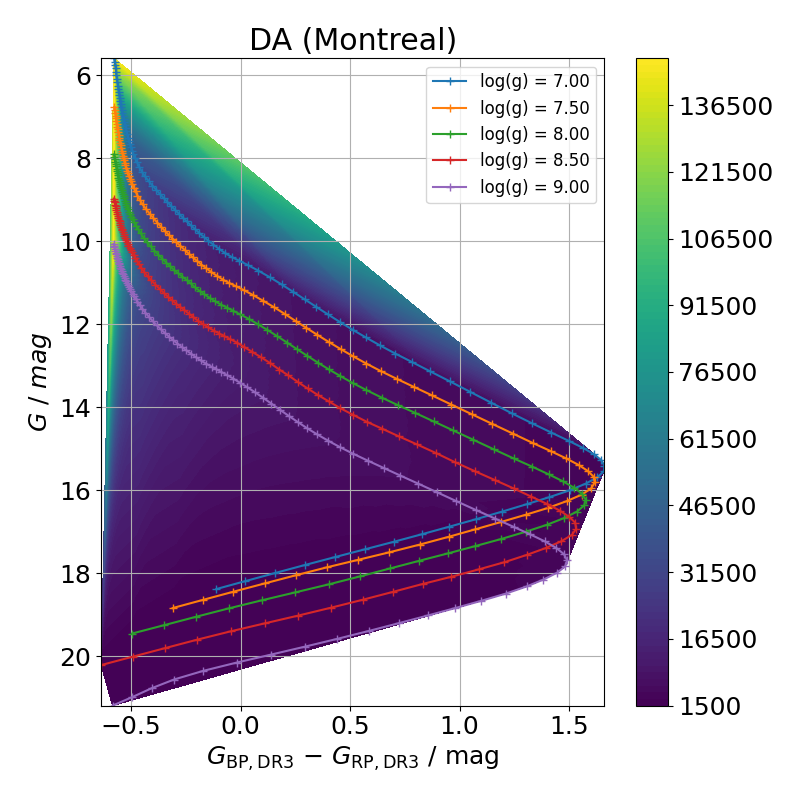
\includegraphics[width=\columnwidth]{DA_cooling_tracks_from_plotter.png}
    \caption{Default figures showing the cooling tracks at different surface
    gravities in the Gaia $G$, $G_{\mathrm{BP}}$ and $G_{\mathrm{RP}}$ filters.
    The colours scale shows the effective temperature.}
    \label{fig:cooling_tracks_default}
\end{figure}

\subsection{Class: \texttt{CoolingModelReader}}
%%%%%%%%%%%%%%%%%%%%%%%%%%%%%%%%%%%%%%%%%%%%%%%%%%%%%%%%%%%%%%%%%%%%%%%%%%%%%%%%
The reader for the 22 cooling models is a little bit more complex because
the outputs from different models are organised differently. These are all
handled in the background and users only need to choose among the models.
Similar to the \verb+AtmosphereModelReader+, after initialisation, the
method \verb+list_cooling_model()+ can be used to retrieve the available models
and then the parameters available for interpolation from those models
can be retrieved using \verb+list_cooling_parameters()+. With the chosen
model name and parameter names, an interpolator can be built using the method
\verb+interp_cm()+, which will use the appropriate formatter and to read
the model files already contained in the package. In this class, the same two
interpolators, \verb+scipy.interpolator.CloughTocher2DInterpolator()+ and 
\verb+scipy.interpolate.RBFInterpolator()+, are available for use. See appendix
for the complete listing of the available models.

(Add description and figure about phase separation and the Q-branch here.)

\section{Photometric fitting}
%%%%%%%%%%%%%%%%%%%%%%%%%%%%%%%%%%%%%%%%%%%%%%%%%%%%%%%%%%%%%%%%%%%%%%%%%%%%%%%%
Photometric fitting can be done by minimizing the $\chi^2$ with any method
supported by \verb+scipy.optimize.minimize()+,
\verb+scipy.optimize.least_squares()+ or with a Markov chain Monte
Carlo method powered by \texttt{emcee}~\citep{2013PASP..125..306F} with the
option to refine the solution with \verb+minimize()+ at the end using the
50-percentile as the initial guess and bounding the fit within N-sigmas
uncertainty limit (user-defined). The H and He atmosphere type has little
effect on the luminosity above around $6000$\,K. Below this, the assumption of
an H atmosphere for an He atmosphere star will lead to an overestimation in
the luminosity, and an underestimation in the distance. Optical spectra are
not particularly useful in distinguishing the atmosphere type, because below
$\sim$\,$5000$\,K, absorption lines starts to disappear. However, the
broad spectral features, namely the collisionally induced absorption, in the
infrared can distinguish the atmosphere type~(see Figure~12 of
\citealt{2017ApJ...848...36B}). Therefore, readers are reminded to pay
particular care when you arrive at a low temperature solution with only
optical data. Since it is only possible to fit for $n-1$ variables, if there
are only two photometric band, it is only possible to fit for a temperature
(and luminosity) with an assumed surface gravity and a known distance. With
three bands, it is mathematically possible to solve for an extra parameter,
i.e. assuming a surface gravity and fit for the temperature and distance,
or assuming a distance and fit for the temperature and surface gravity.
This argument does not apply to fitting with or without interstellar reddening
because it is merely a one-to-one lookup value that is a only a function of
distance. When studying a population of WDs that are fitted for the
distance, we should compare the photometric distance to the distances measured
from other means, e.g. astrometry, spectroscopic distance etc. in order to
assess the bias in the fit~(e.g. Section \textsection3.2.2
in \citealt{2011MNRAS.417...93R}).

%%%%%%%%%%%%%%%%%%%%%%%%%%%%%%%%%%%%%%%%%%%%%%%%%%%%%%%%%%%%%%%%%%%%%%%%%%%%%%%%
The effective temperature (and absolute bolometric magnitude) and the solid
angle of a source can be obtained when the distance is known, through the
relation $\Omega = \pi R^2 / D^2$. In the era of
Gaia~\citep{2021A&A...649A...1G}, most WDs candidates have their parallaxes
measured, and hence the distances derived~\citep{2021AJ....161..147B}. This
allows much more reliable photometric fitting with broadband photometry alone,
as compared to fitting with an assumed surface gravity~(see below). By using
evolutionary model of WDs, the radius and the effective temperature can be
used to obtain the mass (and surface gravity). Even though this is known as
the photometric fitting, and values are almost exclusively reported in
magnitude, the measurement of the apparent brightness is ultimately performed
in electron counts. With good calibration and detector linearity behaviour, it
is sufficiently accurate to treat the uncertainties at the flux level. The
uncertainty in flux measured has a Gaussian-like error that is symmetrical
to both over- and under-estimation of the flux. Unlike with magnitudes,
which is in the logarithmic space of the flux, the uncertainty in magnitude
is no longer symmetrical about the ``central'' value. Thus fitting directly
with magnitude weighted by the magnitude uncertainty leads to a bias: solutions
are biased to be over-luminous. For example, at $\pm0.1$\,mag, the flux
ratios are $1.0965$ and $0.9120$, respectively, corresponding the $(-)8.8\%$
and $(+)9.65\%$ change in the flux in the faint and bright end. This only
narrows down to $(-)0.917\%$ and $(+)0.925\%$ at $\pm0.01\,$mag
level\footnote{A negative change in the magnitude corresponds to increase in
flux.}. This effect becomes visually obvious if one is to perform an MCMC
sampling and inspect the probability distribution functions. For this reason,
in \verb+WDPhotTools+, we fit in flux-space where the linear and symmetrical
approximation of the uncertainty distribution is much more realistic.

\subsection{Mathematical Construction}
%%%%%%%%%%%%%%%%%%%%%%%%%%%%%%%%%%%%%%%%%%%%%%%%%%%%%%%%%%%%%%%%%%%%%%%%%%%%%%%%
we provide three means of fitting, the first two are both finding the minimum
$\chi^2$, with different minimizers. In the following equations, we use $m$ and
$f$ to denote apparent magnitude and flux; and $M$ and $F$ to denote absolute
magnitude and flux. The function to be minimized in these two cases is the
square of the weighted difference between model and observation.
\begin{equation}
    \label{eq:lsq}
    \left(\dfrac{F_{\mathrm{model}, i} - F_{i}}{\sigma_{F, i}}\right)^{2}
\end{equation}
where $F_{\mathrm{model}, i}$ is the model flux in filter $i$, $F$ is the
absolute flux (coming from the observed flux adjusted to it would be if it
were at a distance of $10\,$pc), and $\sigma$ is the combined uncertainty in
the flux and distance which can be found from the formal propagation of
uncertainties from magnitude and distance to flux with
equation \ref{eq:mag_to_flux_err} and
\ref{eq:propagation_of_err}:
\begin{equation}
    \label{eq:mag_to_flux_err}
    \sigma_{f}^{2} = \sigma_{m}^{2} \times \left[ \dfrac{\ln(10) f}{2.5} \right]^{2}
\end{equation}
and
\begin{equation}
    \label{eq:propagation_of_err}
    \sigma_{M}^{2} = \left( \dfrac{\partial M}{\partial m} \sigma_{m} \right)^2 + \left( \dfrac{\partial M}{\partial D} \sigma_{D} \right)^2
\end{equation}
where $D$ and $\sigma_D$ are the distance and the corresponding uncertainty. By
applying the distance-magnitude relation $M = m - 5\log(D)$, it simplifies to
\begin{equation}
    \label{eq:mag_err}
    \sigma_{M}^2 = \sigma^2_{m} + \left[ \dfrac{5 D}{\ln(10)} \right]^2 \sigma_{D}^2.
\end{equation}
Substituting in also the flux-magnitude relation, using the parametrisation
independent of the response of the photometric system: $m - m_{\mathrm{ZP}}=-2.5\log(F/F_{\mathrm{ZP}})$,
we arrive at the $\chi^2$ function to be minimized in the magnitude space weighted
by the formally propagated uncertainties:
\begin{equation}
    \label{eq:chi2}
    \chi^{2} = \dfrac{2.5}{\ln(10)} \sum_{i}\left\{ \dfrac{1}{\sigma_{M, i}} \left[ 10^{\frac{m_{i} - M_{\mathrm{model}, i}}{2.5}} - \dfrac{D^{2}}{100} \right] \right\}
\end{equation}

The third method we provide is to sample the parameter space with an Markov chain
Monte Carlo method. This method more useful in the case when the uncertainties
are large or with missing distance. The likelihood that has to be maximised takes
a similar form to Equation~\ref{eq:chi2}:
\begin{equation}
    \label{eq:likelihood}
    \mathcal{L} = -\dfrac{1}{2} \dfrac{2.5}{\ln(10)} \sum_{i} \left\{ 
    \dfrac{1}{\sigma_{M, i}} \left[ 10^{\frac{m_{i} - M_{\mathrm{model}, i}}{2.5}}  - \dfrac{D^{2}}{100} \right]
    + \ln(2\pi\sigma_i^2) \right\}.
\end{equation}

\subsection{Interstellar Reddening}
%%%%%%%%%%%%%%%%%%%%%%%%%%%%%%%%%%%%%%%%%%%%%%%%%%%%%%%%%%%%%%%%%%%%%%%%%%%%%%%%
When interstellar reddening is included in the calculation, the $\chi^2$
minimisation function becomes
\begin{equation}
    \label{eq:chi2}
    \chi^{2} = \dfrac{2.5}{\ln(10)} \sum_{i}\left\{ \dfrac{1}{\sigma_{M, i}} \left[ 10^{\frac{m_{i} - M_{\mathrm{model}, i} - A_{i}(D)}{2.5}} - \dfrac{D^{2}}{100} \right] \right\};
\end{equation}
and the likelihood function to be maximised becomes
\begin{equation}
    \label{eq:likelihood}
    \mathcal{L} = -\dfrac{1}{2} \dfrac{2.5}{\ln(10)} \sum_{i} \left\{ 
    \dfrac{1}{\sigma_{M, i}} \left[ 10^{\frac{m_{i} - M_{\mathrm{model}, i} - A_{i}(D)}{2.5}}  - \dfrac{D^{2}}{100} \right]
    + \ln(2\pi\sigma_i^2) \right\}.
\end{equation}

%%%%%%%%%%%%%%%%%%%%%%%%%%%%%%%%%%%%%%%%%%%%%%%%%%%%%%%%%%%%%%%%%%%%%%%%%%%%%%%%
where $A_i$ is the total extinction in filter $i$ at distance $D$. In the case
when the distance is known, this is a scale value; when the distance is also
to be fitted, $A$ is not directly provided but instead it is computed from the
$E(B-V)$ at that distance and a choice of $R_{V}$, which is defaulted to $3.1$.
The reddening vector can be applied in two way: (1) it can be approximated by
interpolating over the effective wavelengths of the broadband
filters\footnote{CTIO $UBVRI$, UKIRT $JHKL'$, Gunn $griz$, SDSS $ugriz$,
PS1 $grizy$, LSST $ugrizy$, DES $grizY$ and WFC3 $F218W, F225W$ and $F275W$.
We note that LSST is now renamed as Simonyi Survey Telescope, at the Vera Rubin
Observatory, but it was printed under the former designation in the referenced
article.} available in Table~6 of \citet{2011ApJ...737..103S}; and (2) by
treatment the spectral energy distribution functions more properly, we convolve
the respective filter functions with all the DA
models~\citep{2009ApJ...696.1755T, 2010MmSAI..81..921K} available at the
Spanish Virtual
Observatory\footnote{\url{http://svo2.cab.inta-csic.es/theory/main/}} following
the instructions in \citet{2011ApJ...737..103S}. We have pre-computed the
extinction vector from $Rv = 2.1$ to $5.1$ in $0.5$ step increment, using the
Fitzpatrick extinction law~\citep{1999PASP..111...63F}, for every theoretical
spectrum available over all the filters available from the Montreal synthetic
photometry table. The grid is stored in CSV format and is ready to be
interpolated upon initialisation of this toolkit. The scripts to generate this
table is not included in the standard installation as it is out of scope, it
can be found in the Github repository.

\subsection{Fitting Distance}
%%%%%%%%%%%%%%%%%%%%%%%%%%%%%%%%%%%%%%%%%%%%%%%%%%%%%%%%%%%%%%%%%%%%%%%%%%%%%%%%
Singly evolved WDs are distributed in a small range of surface gravity, with a
mean of $\left<\log(g)\right> = 7.998 \pm 0.011$ in the DA sample in SDSS
DR16~\citep{2021MNRAS.507.4646K}, corresponding to a mean mass of
$\left<\mathcal{M}_i\right> = 0.618 \pm 0.006 \msun$. When studying a large sample of WDs,
fitting the photometric distances for the study of a population is still
useful when reporting an averaged quantity as the final results. The
distributions of the solution are, however, mostly statistical noise and not
representative to the true distribution when both the strongly degenerate
parameters: surface gravity and distance are fitted simultaneous. Equation
\ref{eq:lsq} and \ref{eq:likelihood} are reused in this case, however, the
distance modulus which is a function of distance, is a free parameter to be
fitted.

\subsection{Class: \texttt{WDFitter}}
%%%%%%%%%%%%%%%%%%%%%%%%%%%%%%%%%%%%%%%%%%%%%%%%%%%%%%%%%%%%%%%%%%%%%%%%%%%%%%%%
This class inherits from the \verb+AtmosphereModelReader+. For basic usage,
users are only required to provide the atmospheric type, the magnitudes and
uncertainties in the respective filters. For more advanced usage, other
fine tuning can be performed by providing distance, extinction, independent
variables\footnote{fitting using \testtt{Mbol} and \texttt{Teff} can give slightly
different results due to interpolation.}, choice of interpolator and their
fine-tuning parameters, minimisers and their fine-tuning parameters,
solution refinement within a bounding box (only if \verb+emcee+ was used).
A few arguments are worth extra attention because of the similar terms used
by different methods, we are only pointing out the potential confusion with
the arguments, the detailed usage should be referred to the API document
itself:
\begin{enumerate}
    \item The argument \verb+extinction_convolved+ refers to the used of
    tabulated values from convolving the filter response function with DA
    spectra to compute the extinction corrected for the spectral shape.
    When it is set to \verb+False+, it interpolates the tabulated values
    from \citet{2011ApJ...737..103S}
    \item \verb+kind+ is the kind of interpolation for the extinction.
    \item \verb+logg+ is used if only one independent variable is
    provided.
    \item \verb+method+ sets the choice from the 3 minimizers.
    \item There are 5 keyword arguments that can be used to do fine 
    control over the minimizer and interpolator: \verb+kwargs_for_RBF+,
    \verb+kwargs_for_CT+, \verb+kwargs_for_minimize+,
    \verb+kwargs_for_least_squares+ and \verb+kwargs_for_emcee+.
\end{enumerate}

This class comes with two diagnostic plots. The first one,
\verb+show_best_fit()+ overplots the best fit photometry corrected for the
(fitted) distance (and reddening) with the observed
data~(Figure~\ref{fig:best_fit}). The second one, \verb+show_corner_plot()+,
shows the probability distribution functions from the MCMC
sampling~\ref{fig:emcee_corner} which shows the differences when distance
is provided or not. It is clear from the fit that if the distance is not
provided, the temperature can still be recovered reasonably well because
the SED only changes significantly with distance if the interstellar
reddening is strong. This statement only holds under the assumption that
the WD atmosphere type is typical, photometry is of good quality and a
good number of filters are provided.

\begin{figure}
    \centering
    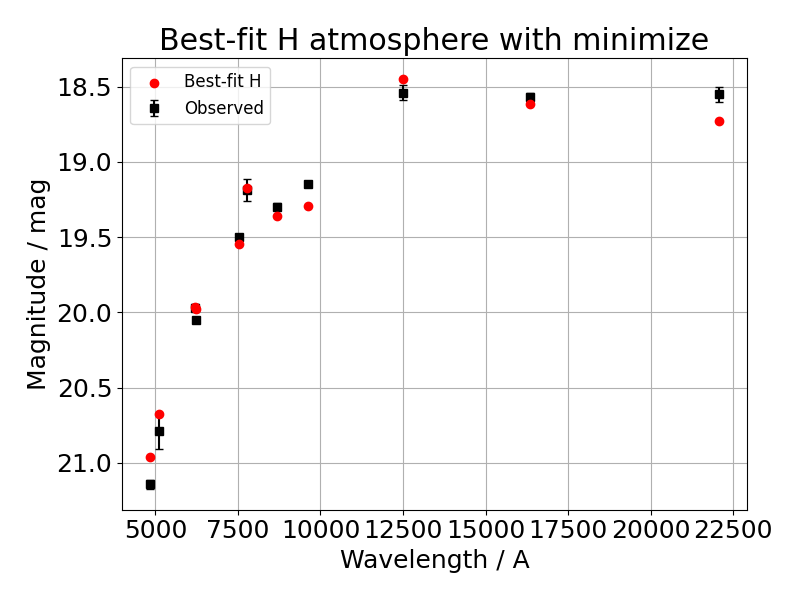
\includegraphics[width=\columnwidth]{PSOJ1801p6254_emcee.png}
    \caption{Best fit DA and DB solutions in for PSO\,J1801+6254~\citep{2020MNRAS.493.6001L}.}
    \label{fig:best_fit}
\end{figure}

\begin{figure}
    \centering
    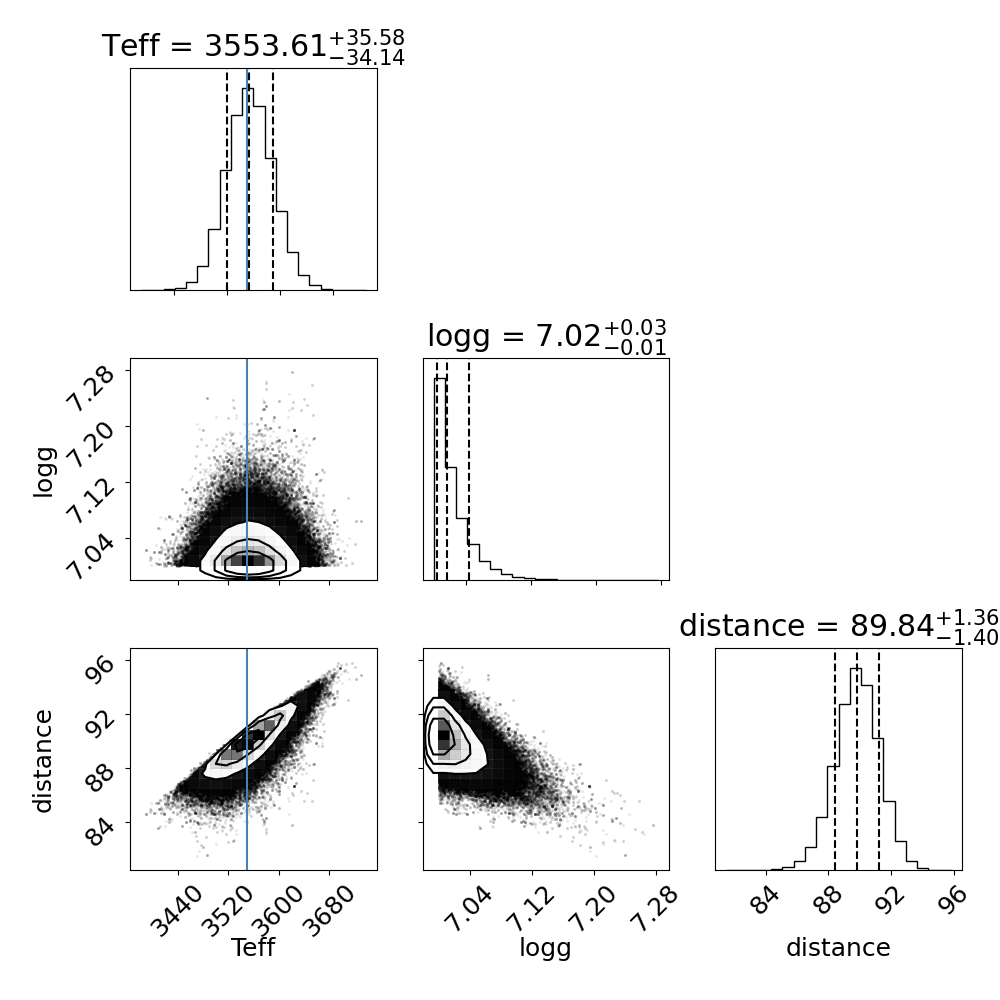
\includegraphics[width=\columnwidth]{PSOJ1801p6254_emcee_corner.png}
    \caption{The corner plot of the sampling using DA model for PSO\,J1801+6254~\citep{2020MNRAS.493.6001L}.}
    \label{fig:emcee_corner}
\end{figure}

%%%%%%%%%%%%%%%%%%%%%%%%%%%%%%%%%%%%%%%%%%%%%%%%%%%%%%%%%%%%%%%%%%%%%%%%%%%%%%%%
\subsection{Comparison against \citet{2021MNRAS.508.3877G}}




\section{White Dwarf Luminosity Function}
%%%%%%%%%%%%%%%%%%%%%%%%%%%%%%%%%%%%%%%%%%%%%%%%%%%%%%%%%%%%%%%%%%%%%%%%%%%%%%%%
WDLF is a common tool for deriving the age of a stellar population. A WDLF is
the number density of WD as a function of luminosity, it is an evolving
function with time. Its shape and normalisation determined from only a few
parameters. \citet{1987ApJ...315L..77W} compared an observed WDLF derived from
the Luyten Half-Second~(LHS) catalogue with a theoretical WDLF to obtain an
estimate of the age of the Galaxy for the first time with this technique.
\citet{1990ApJ...352..605N} examined WDLFs with various SFH scenarios. They
showed that WDLF is a sensitive probe of the star formation history~(SFH) as
it shows signatures of irregularities in the SFH such as bursts and lulls.
\citet{2013MNRAS.434.1549R} took it further to address this inverse problem
mathematically and showed some success in recovering the SFH of the solar
neighbourhood when compared against SFH computed from other methods. By
decomposing the disks and halo components of the Milky Way, we can have an
independent view of the past star formation history revealed by only the
WD populations, where they are most useful in deriving the SFH of old
stellar populations~\citep{2011MNRAS.417...93R, 2017ASPC..509...25L}.


%%%%%%%%%%%%%%%%%%%%%%%%%%%%%%%%%%%%%%%%%%%%%%%%%%%%%%%%%%%%%%%%%%%%%%%%%%%%%%%%
The mathematical construction of a WDLF is intuitively straightforward: stars
were formed in a distribution of mass~($\mathcal{M}_i$), described by the initial
mass function~(IMF, $\phi$). Then, they spend their lifetime carrying out
nuclear burning~($t_{\mathrm{MS}}$), the time they spend depends mainly on
their mass. Towards the end stage of stellar evolution stars shed most of the
atmosphere, which is modelled by the initial-final mass relation~(IFMR,
$\zeta$). Once they have become WDs, all is left is to know how long it has
been cooling~($t_{\mathrm{cool}}$) in order to reach the current
luminosity~($M_\mathrm{bol}$). The heavy duty of these computations
are coming from interpolation of pre-computed lookup tables. The important
part of this work is to carefully interpolate and integrate over the model
grids, because they are both susceptible to significant rounding errors given
the huge dynamic ranges the variables cover. For example, in case of a simple
star burst of $\mathcal{O}(10^6)$\,yrs, it requires a relative error
tolerance of $10^{-10}$ in order to integrate properly for an old population.

%%%%%%%%%%%%%%%%%%%%%%%%%%%%%%%%%%%%%%%%%%%%%%%%%%%%%%%%%%%%%%%%%%%%%%%%%%%%%%%%
The integral for a WDLF when parameterised with bolometric magnitude (as
opposed to luminosity) can be written as

\begin{equation}
    n(M_{\mathrm{bol}}) = \int_{\mathcal{M}_l}^{\mathcal{M}_u}
        \tau(M_\mathrm{bol}, \mathcal{M}_f)
        \psi(T_0, M_\mathrm{bol}, \mathcal{M}_i, m, Z)
        \phi(\mathcal{M}_i) d\mathcal{M}_i
\end{equation}
where $n$ is the number density, $\tau$ is the inverse cooling rate, $\psi$ is
the relative star formation rate, $\phi$ is the initial mass function; and their
dependent variables: $M_\mathrm{bol}$ is the absolute bolometric
magnitude, $\mathcal{M}_f$ is the WD mass, $T_0$ is the look-back time, $\mathcal{M}_i$ is
the progenitor MS mass, $Z$ is the metallicity, $\mathcal{M}_l$ is the minimum
progenitor MS mass that could have singly evolved into a WD in the given time,
and $\mathcal{M}_u$ is the maximum progenitor MS mass.

%%%%%%%%%%%%%%%%%%%%%%%%%%%%%%%%%%%%%%%%%%%%%%%%%%%%%%%%%%%%%%%%%%%%%%%%%%%%%%%%
The inverse cooling rate
\begin{equation}
    \tau(M_\mathrm{bol}, \mathcal{M}_f) = \dfrac{dt_{\mathrm{cool}}}{dM_\mathrm{bol}} \left( M_\mathrm{bol}, \mathcal{M}_f \right)
\end{equation}
is a quantity taken from the pre-computed grid of cooling models. 

The relative star formation rate is expressed as a function of look-back time,
\begin{align}
    &\psi(T_0, M_\mathrm{bol}, \mathcal{M}_i, \mathcal{M}_f, Z) =\\
    &\qquad\psi\left[T_0 - t_{\mathrm{cool}}\left(M_\mathrm{bol}, \mathcal{M}_f\right) - t_{\mathrm{MS}}\left(\mathcal{M}_i, Z\right)\right].
\end{align}
The absolute normalisation is not needed when the total stellar mass is coming
from observations; the theoretical WDLF only needs to multiply with a
constant (the total number density) to account for the normalisation.

%%%%%%%%%%%%%%%%%%%%%%%%%%%%%%%%%%%%%%%%%%%%%%%%%%%%%%%%%%%%%%%%%%%%%%%%%%%%%%%%
The IFMR takes a simple form of
\begin{equation}
    \mathcal{M}_f = \zeta(\mathcal{M}_i),
\end{equation}
although there are evidence that more metal rich stars lose more
envelope~\citep{2007ApJ...671..761K}, there is insufficient empirical data to
derive a IFMR at metallicity much lower or higher than solar abundance.

\subsection{Initial Mass Function (IMF)}
%%%%%%%%%%%%%%%%%%%%%%%%%%%%%%%%%%%%%%%%%%%%%%%%%%%%%%%%%%%%%%%%%%%%%%%%%%%%%%%%
The IMF has little effect on the WDLF because of their similarity over the mass
range that stars could have become WDs. Nevertheless, we are providing three
of the most used IMFs, they differ very slightly when the mass is less than
$1\,\msun$. The effect can appear in the bright end of a WDLF for an old
population. A callable function can be supplied as a manual IMF. This lists the
four options that are available:

\begin{enumerate}
    \item \citet{2001MNRAS.322..231K} is a three-part power law that only the
    more massive two are of relevance to this work, with
    $\xi(\mathcal{M}_i) = \mathcal{M}_i^{-\alpha}$ where
    \begin{equation}
        \alpha =
        \begin{cases}
            0.3, \quad \mathcal{M}_i \leq 0.08\,\msun\\
            1.3, \quad 0.08 \leq \mathcal{M}_i \leq 0.5\,\msun\\
            2.3, \quad \mathcal{M}_i \geq 0.5\,\msun.
        \end{cases}
    \end{equation}
    \item \citet{2003PASP..115..763C} shares the same power law with
    \citet{2001MNRAS.322..231K} for mass above $1\,\msun$, at lower mass,
    the IMF follows a log-normal form with
    \begin{equation}
        \xi(\mathcal{M}_i) = \dfrac{0.158^{+0.051}_{-0.046}}{\mathcal{M}_i \ln(10)} \times
            \exp{\left\{\dfrac{\left[\log(\mathcal{M}_i) - \log\left(0.079^{-0.016}_{+0.021}\right)\right]^2}{2 \times (0.69^{-0.01}_{+0.05})^2}\right\}}
    \end{equation}
    \item \citet[][including binary]{2003PASP..115..763C} also consider the correction for binaries which gives a much shallower IMF at the low mass end
    \begin{equation}
        \xi(\mathcal{M}_i) = \dfrac{0.086}{\mathcal{M}_i \ln(10)} \times
            \exp{\left\{\dfrac{\left[\log(\mathcal{M}_i) - \log\left(0.022\right)\right]^2}{2 \times (0.57)^2}\right\}}
    \end{equation}
    \item Manual provided interpolated function that return the initial mass density as list or array (even if a single point is returned).
\end{enumerate}

\subsection{Star Formation History (SFH)}
%%%%%%%%%%%%%%%%%%%%%%%%%%%%%%%%%%%%%%%%%%%%%%%%%%%%%%%%%%%%%%%%%%%%%%%%%%%%%%%%
The SFH has one of the strongest effect on the shape and normalisation of a
WDLF. The default profiles are only three types of simple form SFH, however,
exponential decay profile with an appropriate decay coefficient should give a
first good guess for a disk population, while a burst profile would be useful
for studying open or globular clusters. All three profiles are controlled by
a few simple parameters, and the fourth option is to provide a callable
function of star formation rate as a function of look back time:
(1)~\textit{Constant} profile depends only on the age of the population,
i.e. the look back time since the beginning of star formation,
and \textbf{not} the time since the first WD was formed. (2)~\textit{Burst}
profile which depends on the onset of start formation as well as the duration
of a constant burst of star formation. (3)~An ~\textit{exponentially decaying}
profile that is government by the onset of star formation, the decay coefficient
and the duration of the star formation. By default it continues to decay
indefinitely. (4)~A ~\textit{manually provided callable function} that can take
any form, though users should be careful with the extrapolation setting,
smoothly extrapolated value or zero should be returned. In case of \verb+NaN+
or $\pm$inf being returned, we set the value to zero.

%%%%%%%%%%%%%%%%%%%%%%%%%%%%%%%%%%%%%%%%%%%%%%%%%%%%%%%%%%%%%%%%%%%%%%%%%%%%%%%%
Since we normalise the output WDLF by the total integrated number density at
all luminosities, the absolute normalisation of the input SFH is discarded when
provided manually.

\subsection{Main Sequence Lifetime}
%%%%%%%%%%%%%%%%%%%%%%%%%%%%%%%%%%%%%%%%%%%%%%%%%%%%%%%%%%%%%%%%%%%%%%%%%%%%%%%%
The MS lifetime has a strong effect on the bright end of a WDLF because the hot
WDs spent most of their time since star formation as their progenitors.
However, the MS lifetime has decreasing impact on the WDLF as we move towards
the fainter end where WDs cooling time dominates over the MS lifetime. There is
also a metallicity dependency on the MS lifetime. From the PARSEC
models~\citep{2013EPJWC..4303001B}, extremely metal poor $1\,\msun$ star with
$Z=0.001$ and solar-metallicity star with $Z=0.017$ take $\sim$\,$6$\,Gyr and
$\sim$\,$11$\,Gyr to go through the MS stage, respectively. Furthermore,
the mass loss during the late stage of stellar evolution also differ at
different metallicity. However, we are only providing solar-metallicity
MS lifetime model because the IFMR models are all derived from WDs that
were once progenitors with an unknown metallicity, and the solar metallicity
is only slightly more abundant than the average metallicity in the Milky Way
in the vicinity of the Sun. The following MS lifetime models are interpolated and
the option of providing a callable function is also a possible form as input:

\begin{enumerate}
    \item \citet{2013EPJWC..4303001B}
    \item \citet{2016ApJ...823..102C}
    \item Manual
\end{enumerate}

\subsection{Initial-Final Mass Relation (IFMR)}
%%%%%%%%%%%%%%%%%%%%%%%%%%%%%%%%%%%%%%%%%%%%%%%%%%%%%%%%%%%%%%%%%%%%%%%%%%%%%%%%
Human civilisation has existed a mere few thousand years, and modern astronomy
(with digital aid) is no more than a hundred. We do not have direct
observations on the total mass loss of a star at the end stage of stellar
evolution. It depends on observations of WDs and giants in clusters and
iteratively comparing with stellar evolution models. There are a number of
IFMRs available from studying globular clusters~\citep{2004A&A...420..515M,
2009ApJ...705..408K}, open clusters~\citep{2009ApJ...693..355W,
2016ApJ...818...84C}, wide MS-WD binaries~\citep{2008A&A...477..213C,
2012ApJ...746..144Z, 2018ApJ...860L..17E}, wide turnoff/subgiant-WD
binaries~\citep{2021ApJ...923..181B}, wide WD-WD
binaries~\citep{2015ASPC..493..325C, 2015ApJ...815...63A, 2018ApJ...866...21C}.
We have chosen six (plus three with two-part fitting) works that have a
good mass coverage to be included in this work, and just like the other
functions above, a manualy provided callable function is also accepted:

\begin{enumerate}
    \item \citet{2008MNRAS.387.1693C} -- this work reanalysed all the known WDs in clusters and MS-WD binaries homogeneously by using a single stellar evolution model and a single WD cooling model. The sample covers a mass range of $1.5-6.4\,\msun$, giving a best-fit IFMR of
    \begin{equation}
        \mathcal{M}_f = (0.117 \pm 0.004)\,\mathcal{M}_i + (0.384 \pm 0.011)\,\msun.
    \end{equation}
    \item \citet[][two-part]{2008MNRAS.387.1693C} -- in the same work, they also fitted with a 2-part IFMR with a break point at $2.7\,\msun$, which gives a steeper relation at the high mass end with
    \begin{equation}
        \mathcal{M}_f = \begin{cases}
                  (0.096 \pm 0.005)\,\mathcal{M}_i + (0.429 \pm 0.015)\,\msun,\\
                  \qquad(\mathcal{M}_i \leq 2.7\,\msun)\\
                  (0.137 \pm 0.007)\,\mathcal{M}_i + (0.318 \pm 0.018)\,\msun,\\
                  \qquad(\mathcal{M}_i \geq 2.7\,\msun)
              \end{cases}
    \end{equation}
    \item \citet{2009ApJ...692.1013S} -- by using 10 (young) open clusters, this relation is probing the high mass end of the population that can turn into WDs. They, however, do not have enough time for the lower mass stars to evolve into WDs hence this relation is unconstrained below $1.7\,\msun$ and we extrapolate if the given initial mass is below $1.7\,\msun$. The upper limit of the data set is $8.5\,\msun$:
    \begin{equation}
        \mathcal{M}_f = 0.084 \mathcal{M}_i \pm 0.466\,\msun.
    \end{equation}
    \item \citet[][two-part]{2009ApJ...692.1013S} -- in the same work, they also fitted with a 2-part IFMR with a break point at $4\,\msun$.
    \begin{equation}
        \mathcal{M}_f = \begin{cases}
                  0.134\,\mathcal{M}_i + 0.331\,\msun, &1.7\,\msun \leq \mathcal{M}_i \leq 4.0\,\msun\\
                  0.047\,\mathcal{M}_i + 0.679\,\msun, &\mathcal{M}_i \geq 4.0\,\msun
              \end{cases}
    \end{equation}
    \item \citet{2009ApJ...693..355W} is an extension to \citet{2009ApJ...692.1013S} by including M41 to the collection of open clusters, covering a reliable mass range of $1.25-8.0\,\msun$,
    \begin{equation}
        \mathcal{M}_f = (0.129 \pm 0.004) \mathcal{M}_i + (0.339 \pm 0.015)\,\msun.
    \end{equation}
    \item \citet{2009ApJ...705..408K} reanalysed with all the available open clusters covering a mass range of $1.1-6.5\,\msun$ to give a relation of
    \begin{equation}
        \mathcal{M}_f = (0.109 \pm 0.007) \mathcal{M}_i + (0.428 \pm 0.025)\,\msun.
    \end{equation}
    \item \citet[][extended]{2009ApJ...705..408K} includes also the WDs from the globular cluster, M4, to give a shallower relation.
    \begin{equation}
        \mathcal{M}_f = (0.101 \pm 0.006) \mathcal{M}_i + (0.463 \pm 0.018)\,\msun.
    \end{equation}
    However, having only metal richer open cluster data at the high mass end and only the metal poor globular cluster data at the low mass end is likely to lead to a shallower fit expected due to the metallicity dependency in the total mass loss at the late stage of stellar evolution.
    \item \citet{2018ApJ...866...21C} has fitted and compared various theoretical and empirical models, we are only providing the 3-part-solution that the authors preferred, which is based on the MIST stellar evolution model,
    \begin{equation}
        \mathcal{M}_f = \begin{cases}
                  (0.080 \pm 0.016)\,\mathcal{M}_i + (0.489 \pm 0.030)\,\msun,\\
                  \qquad(0.83\,\msun \leq \mathcal{M}_i \leq 2.85\,\msun)\\
                  (0.187 \pm 0.061)\,\mathcal{M}_i + (0.184 \pm 0.199)\,\msun,\\
                  \qquad(2.85\,\msun \leq \mathcal{M}_i \leq 3.6\,\msun)\\
                  (0.107 \pm 0.016)\,\mathcal{M}_i + (0.471 \pm 0.077)\,\msun,\\
                  \qquad(3.6\,\msun \leq \mathcal{M}_i \leq 7.2\,\msun)\\
              \end{cases}
    \end{equation}
    \item \citet{2018ApJ...860L..17E} reports the relations by fitting the colour-magnitude diagram of the clean Gaia DR2 WD sequence. It is a 5-point piecewise-linear function going through the following (initial mass, final mass) coordinates: $(0.95, 0.5^{+0.01}_{-0.01})$, $(2.75^{+0.36}_{-0.31}$, $0.67^{+0.02}_{-0.02})$, $(3.54^{+0.55}_{-0.43}$, $0.81^{+0.03}_{-0.03})$, $(5.21^{+1.06}_{-0.71}$, $0.91^{+0.10}_{-0.03})$ and $(8.0, 1.37^{+0.06}_{-0.21})$.
    \item Manually provided interpolated function that return the final mass as list or array (even if a single point is returned).
\end{enumerate}


\subsection{Cooling Models}
%%%%%%%%%%%%%%%%%%%%%%%%%%%%%%%%%%%%%%%%%%%%%%%%%%%%%%%%%%%%%%%%%%%%%%%%%%%%%%%%
Most of the internal energy of a WD is the residual heat from the progenitor
once it passed the planetary nebula phase. However, there are various physical
processes that can provide an appreciable amount of energy and govern the
cooling rate of a WD at different stages. Following the time sequence in which
the physical processes that has direct effects to the photo-luminosity: (1)~in
the first $10^8-10^9$ years, \textit{shell burning of hydrogen} via pp-chain
can contribute up to $30\%$ of the total luminosity~\citep{2010ApJ...717..183R}.
(2)~\textit{Neutrino losses} -- contribute to a significant fraction of energy
loss in the early time of WDs when they were still hot, in the case of massive
WDs, neutrino bremsstrahlung effect must also be taken into account
\citep{1994ApJ...425..222H, 1996ApJS..102..411I}. (3)~\textit{Gravitational
settling} of\ $^{22}$Ne in intermediate to massive WDs releases sufficient
gravitational potential energy to prolong the cooling
times~\citep{2002ApJ...580.1077D, 2008ApJ...677..473G, 2010ApJ...719..612A}.
The heavier\ $^{22}$Ne relative to the environment that is dominated by carbon,
oxygen and nitrogen leads to a slow settling towards the core. This effect is
the most obvious in the old and metal-rich systems, such as NGC
6791~\citep{2010Natur.465..194G, 2008ApJ...678.1279B}. (4)~In the late time of
the WD evolution, convection plays a significant role in slowing down the
cooling. As temperature decreases, the convective zone grows deeper into the
interior and eventually reaches the degenerate core~(see Figure~11
from~\citealt{2010A&ARv..18..471A}). This efficiently replenish the energy
radiated away from the photosphere, thus this process known as the
\textit{convective coupling}, modifies the relations between the WD luminosity
and core temperature~\citep{1989ApJ...347..934D, 2001PASP..113..409F}.
(5)~\textit{Crystallisation} occurs as the non-degenerate ions evolve from gas
to fluid and eventually solid. The liquid-solid transition releases latent
heat that slows down the cooling process. This also couples with the release
of gravitational energy associated with changes in the carbon-oxygen
profile~\citep{1997ApJ...486..413S} when the heavier oxygen-rich crystals
displace carbon as a result of gravitational settling. Depending on the
changes in the carbon-oxygen abundance profile, and the choice of phase
diagram of a carbon-oxygen mixture, it modifies the rate of cooling and this
specific effect is colloquially known as the (6)~\textit{Phase Separation}
effect. (7)~\textit{Coulomb Interactions} modify the thermodynamical
properties of the ionic gas, in particular the specific heat. Its strength is
determined by the Coulomb coupling parameters. At first, the parameter is
small, it slowly increases as an WD cools and the ions begins to change for
gas to liquid and eventually forming lattice. This releases latent heat that
contribute to $\sim$\,$5\%$ of the total luminosity~\citep{1976A&A....51..383S}.
At late time, few modes of the lattice are excited, the heat capacity drops
according to the Debye law, this results in enhanced cooling. This process
kicks in after $10^9$\,yr for a $1.0\,\msun$ WD and over a Hubble time for a
$0.5\,\msun$ WD.

\subsection{Class: \texttt{WDLF}}
%%%%%%%%%%%%%%%%%%%%%%%%%%%%%%%%%%%%%%%%%%%%%%%%%%%%%%%%%%%%%%%%%%%%%%%%%%%%%%%%
This class inherits from the \verb+AtmosphereModelReader+ and the
\verb+CoolingModelReader+.

A \texttt{WDLF} object takes requires six models for computation: (1)~IMF,
(2)~IFMR, (3)~MS lifetime model, and (4-6) low, intermediate and high mass WD
cooling models. We have included 22 cooling models from 11 works that cover
different parts of the parameter space. See Table~\ref{tab:cooling_models} for
the details of each model. This comes with a diagnostic plot to inspect all
the input models: the IMF, the SFH, the MS lifetime as a function of mass,
the IFMR, and the cooling model in two formats: bolometric magnitude as a
function of age, and the rate of change of the bolometric magnitude as a
function of age~(Figure~\ref{fig:input_model}).

\begin{figure*}
    \centering
    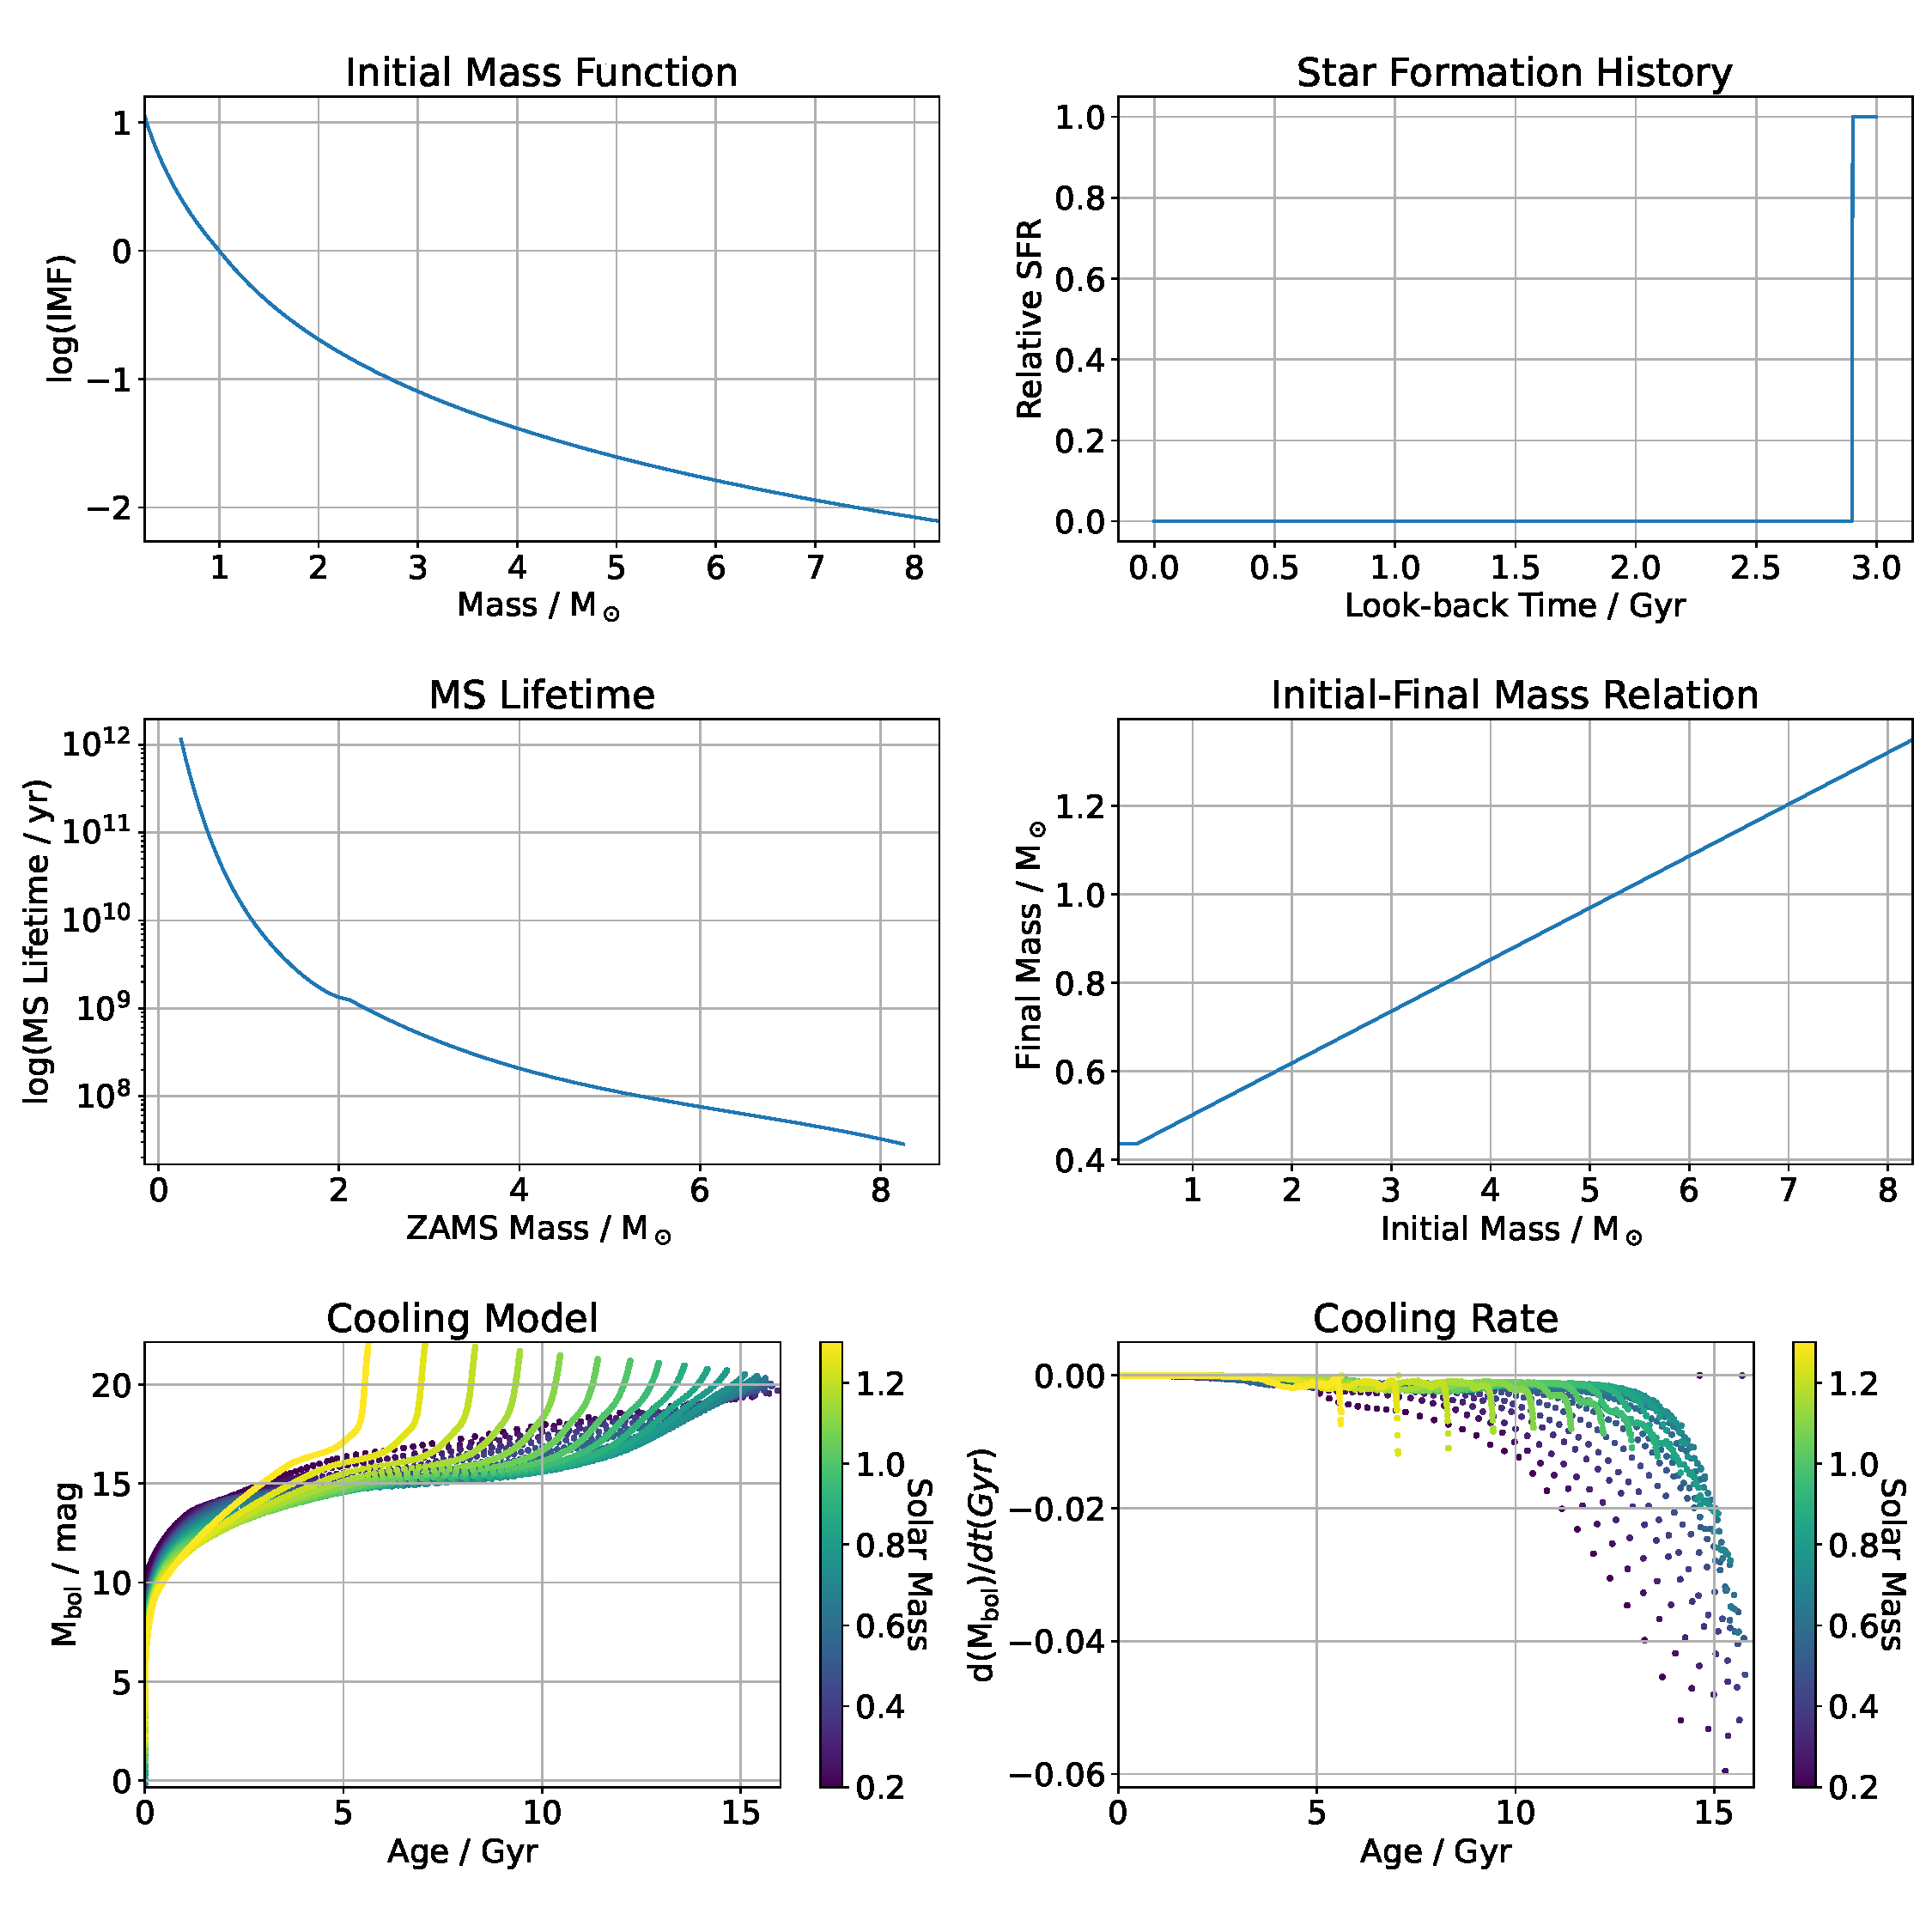
\includegraphics[width=\textwidth]{input_model.pdf}
    \caption{Caption}
    \label{fig:input_model}
\end{figure*}

In the following comparisons, the default configuration uses the (1)~IMF
from \citet{2003PASP..115..763C} for single stars, (2)~IFMR from
\citet{2008MNRAS.387.1693C}, and (3)~cooling models from the Montreal group,
and (4)~SFH is a star burst of $10^8$ starting at the labelled time.
While comparing the theoretical WDLFs, we are altering one variable at a time.
All WDLFs are normalised at $10$\,mag to a log-number density of $0.0$.

\subsubsection{Star Formation History}
%%%%%%%%%%%%%%%%%%%%%%%%%%%%%%%%%%%%%%%%%%%%%%%%%%%%%%%%%%%%%%%%%%%%%%%%%%%%%%%%
This WDLFs with various star formation history are shown in
Figure~\ref{fig:compare_sfr_age_type}. The bright edge of the WDLFs line up
almost perfectly because WDs arrive at the corresponding bolometric magnitudes
at a constant rate. The gradient is most sensitive to a time-dependent
variable, for example, a change in the SFR. The sudden increase in the number
density at $M_\mathrm{bol}=14.5$ corresponds to the slow down in the cooling
due to crystallisation that releases a significant amount of heat. This bump
is the most prominent in the star burst profile at $6$\,Gyr old because WDs
with $\sim0.8-1.0\,\msun$ have the the lowest cooling rates, they corresponds
to $3-5\msun$ ZAMS mass that spends $0.1-0.5$\,Gyr in the MS and $5-6$\,Gyr
to reach $14.5$\,mag~($\sim 5500$\,K, \citealp{2019ApJ...876...67B}). The
detailed description of the shape of the WDLFs due to various cooling
mechanism should be referred to  Figure~5 and Section~3
of \citep{2001PASP..113..409F}.

\begin{figure}
    \centering
    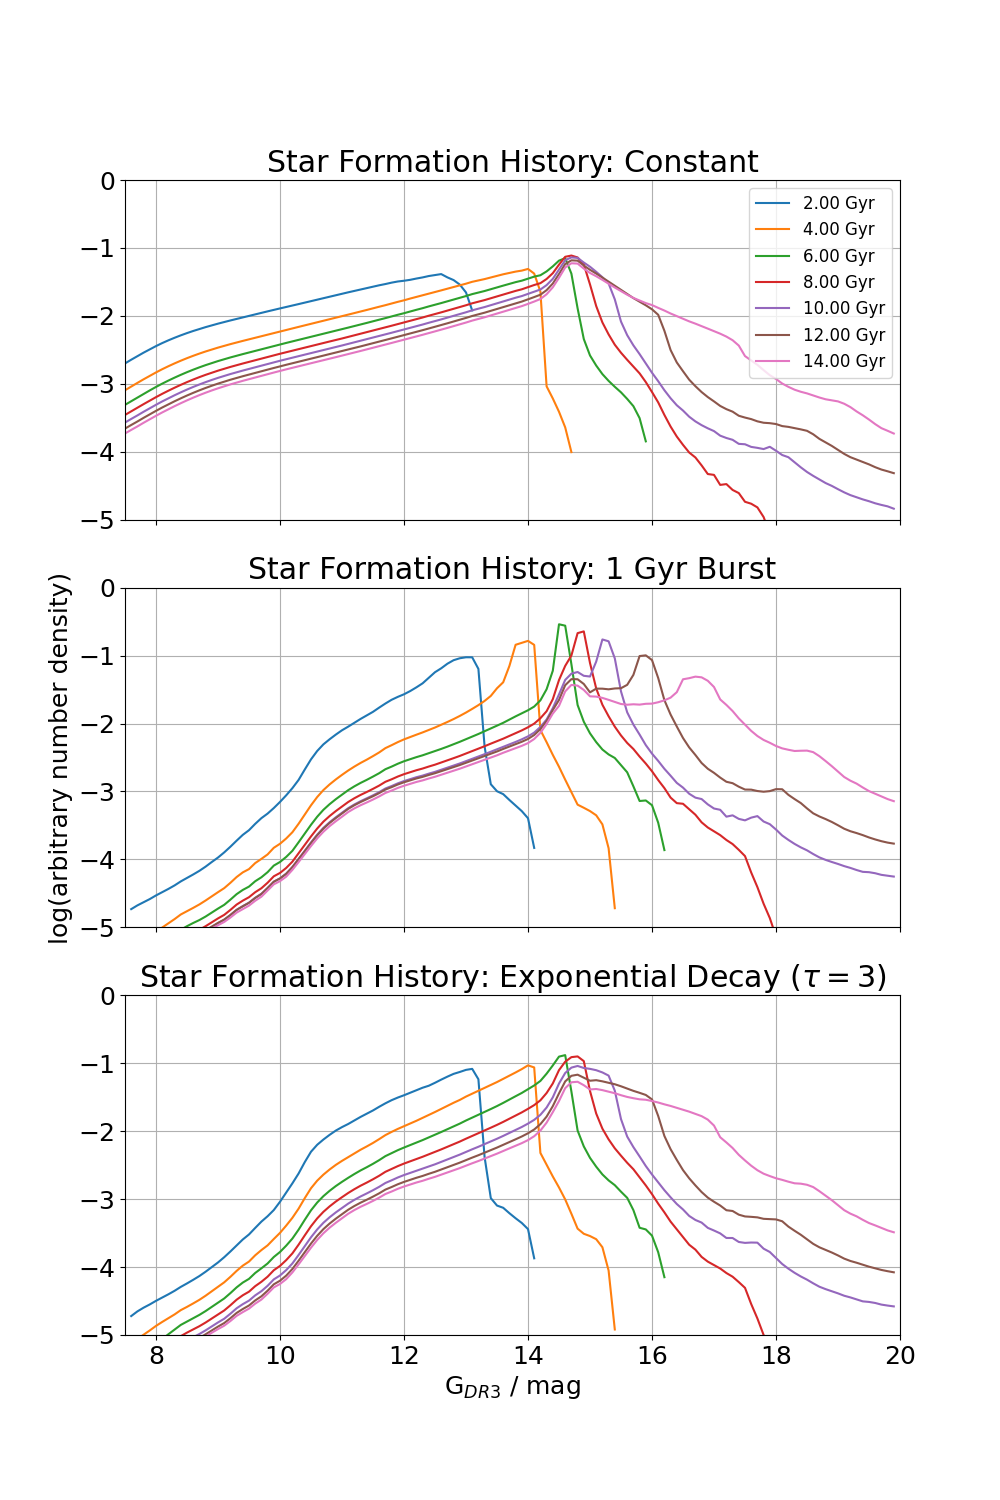
\includegraphics[width=\columnwidth]{wdlf_compare_sfr.png}
    \caption{Comparing WDLFs with the three default types of star formation
    history from $2$ to $14\,$Gyr in increment of $2$\,Gyr.}
    \label{fig:compare_sfr_age_type}
\end{figure}

\subsubsection{Initial Mass Functions}
%%%%%%%%%%%%%%%%%%%%%%%%%%%%%%%%%%%%%%%%%%%%%%%%%%%%%%%%%%%%%%%%%%%%%%%%%%%%%%%%
There is a very weak dependency on the IMF in because the three IMFs are only
different at mass below $1\,\msun$, which has a MS lifetime of $11.72$\,Gyr.
Hence, we only start to see a difference in the WDLF at ages above
$11$\,Gyr~(Figure~\ref{fig:wdlf_compare_imf}. The IMFs only diverge significant
well into the M-dwarf brown dwarf regime,at a computed age of $15$\,Gyr
we are only including stars with ZAM masses as low as $\sim$ $0.96\,\msun$.
Nevertheless, if a metal poor MS lifetime model is used, this can change the
picture slightly, although, the effect would still be much smaller than another
or uncertainties in other models and observations.

\begin{figure}
    \centering
    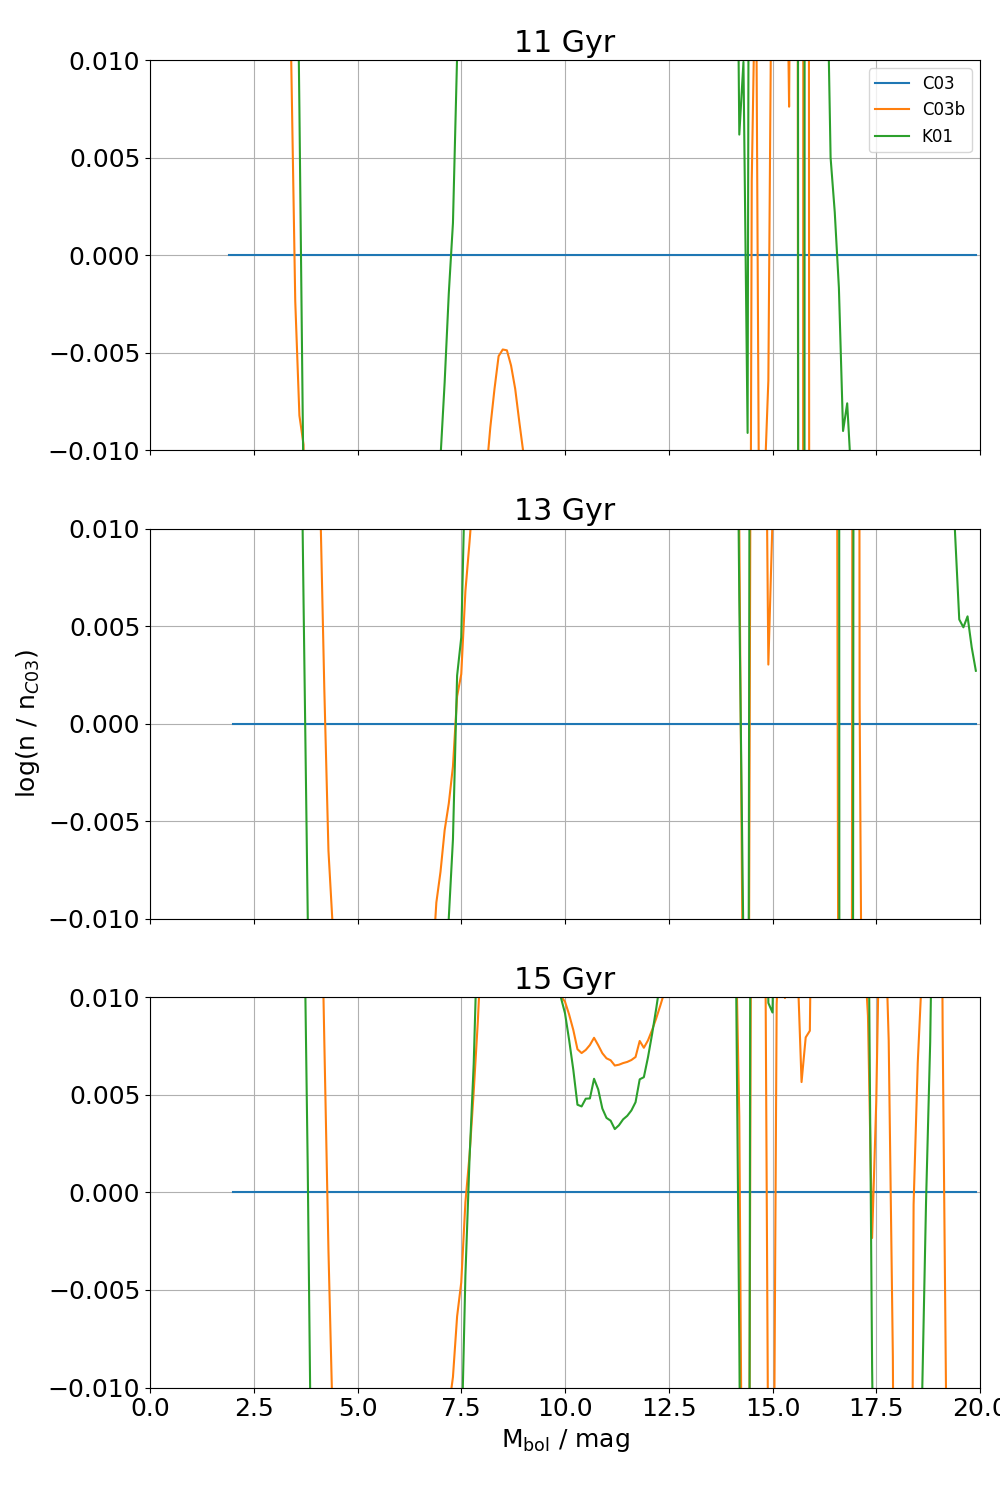
\includegraphics[width=\columnwidth]{wdlf_compare_imf.png}
    \caption{Comparing WDLFs with different input IMFs.}
    \label{fig:wdlf_compare_imf}
\end{figure}

\subsubsection{Initial-Final Mass Relations}
%%%%%%%%%%%%%%%%%%%%%%%%%%%%%%%%%%%%%%%%%%%%%%%%%%%%%%%%%%%%%%%%%%%%%%%%%%%%%%%%
The WDLFs in the range of $9$--$14$\,mag line up almost perfectly at any age.
This is because WDs at any typical mass does not have any mass-dependent
physical phenomenon that affects the WD evolution. They all cool similarly at
roughly the same rate across the mass range of the models. 

Figure~\ref{fig:wdlf_compare_ifmr}
\begin{figure*}
    \centering
    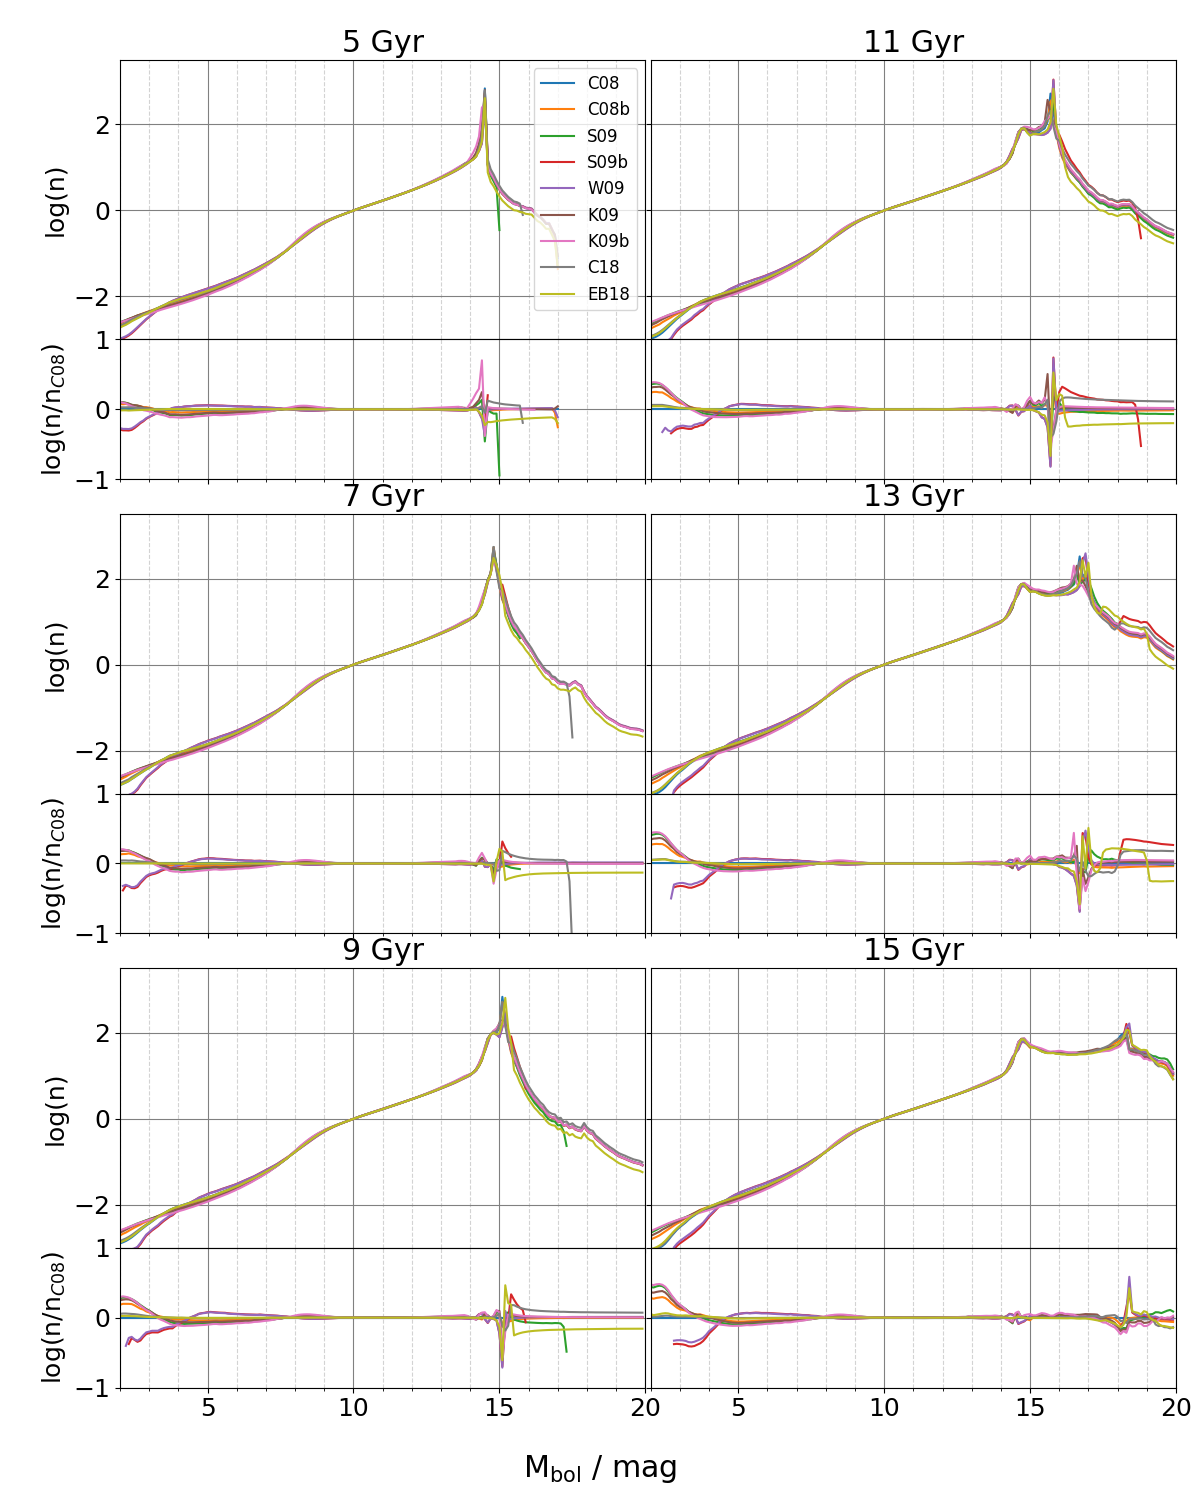
\includegraphics[width=\textwidth]{wdlf_compare_ifmr.png}
    \caption{Comparing WDLFs with different input IFMRs.}
    \label{fig:wdlf_compare_ifmr}
\end{figure*}

\subsubsection{Cooling Models}
%%%%%%%%%%%%%%%%%%%%%%%%%%%%%%%%%%%%%%%%%%%%%%%%%%%%%%%%%%%%%%%%%%%%%%%%%%%%%%%%
Figure~\ref{fig:wdlf_compare_da_cooling_models}
\begin{figure*}
    \centering
    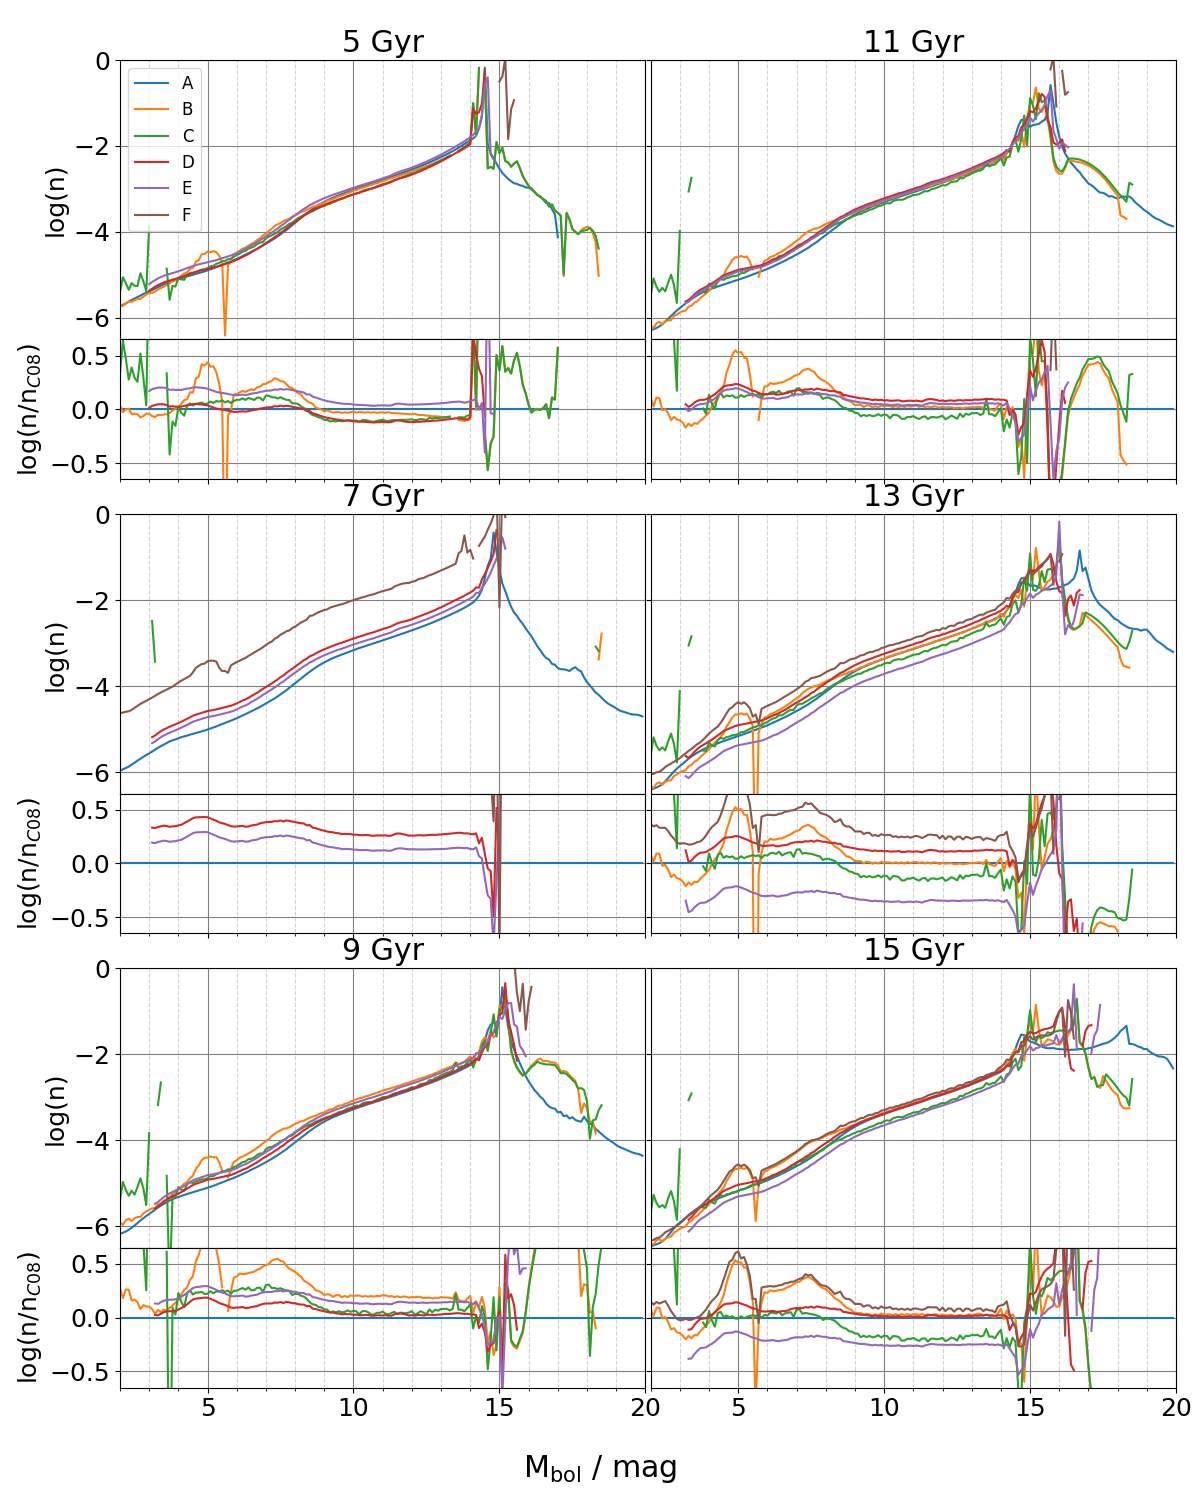
\includegraphics[width=\textwidth]{wdlf_compare_da_cooling_models.png}
    \caption{Comparing WDLFs with different input cooling models.}
    \label{fig:wdlf_compare_da_cooling_models}
\end{figure*}

\begin{table*}
    \centering
    \begin{tabular}{c|c|c|c|c|c|c|c}
        Reference             &    Low     & Intermediate &    High    &  Core & Atmosphere &           Mass Range $\left(\mathcal{M}_f/\msun\right)$ & Extra Notes \\\hline\hline

        \multicolumn{8}{c}{Montreal Model} \\\hline
        \citet{2020ApJ...901...93B} & \checkmark &  \checkmark  & \checkmark &    CO &      DA/DB &            $0.2-1.3$             & -- \\
        &&&&&&&\\

        \multicolumn{8}{c}{La Plata Models} \\\hline
        \citet{2007MNRAS.382..779P} & \checkmark &      --      &     --     & He/CO &         DA &          $0.187-0.448$           & -- \\
        \citet{2009ApJ...704.1605A} & \checkmark &      --      &     --     &    He &         DA &          $0.220-0.521$           & -- \\
        \citet{2010ApJ...717..183R} &     --     &  \checkmark  &     --     &    CO &         DA &          $0.505-0.934$           & $Z=0.001-0.01$ \\
        {\citet{2015A&A...576A...9A}} &     --     &  \checkmark  &     --     &    CO &         DA &          $0.506-0.826$           & $Z=0.0003-0.001$ \\
        {\citet{2017A&A...597A..67A}} & \checkmark &  \checkmark  &     --     &    CO &         DA &          $0.434-0.838$           & $Y=0.4$ \\
        \citet{2017ApJ...839...11C} &     --     &  \checkmark  &     --     &    CO &         DB &           $0.51-1.0$             & -- \\
        {\citet{2007A&A...465..249A}} &     --     &      --      & \checkmark &   ONe &         DA &           $1.06-1.28$            & -- \\
        {\citet{2019A&A...625A..87C}} &     --     &      --      & \checkmark &   ONe &      DA/DB &           $1.10-1.29$            & -- \\
        &&&&&&&\\

        \multicolumn{8}{c}{BaSTI Models} \\\hline
        \citet{2010ApJ...716.1241S} &     --     &  \checkmark  & \checkmark &    CO &      DA+DB &           $0.54-1.2$             & With/Without Phase Separation\\
        &&&&&&&\\

        \multicolumn{8}{c}{MESA Models} \\\hline
        \citet{2018MNRAS.480.1547L} &     --     &      --      & \checkmark & CO/Ne &      DA/DB &          $1.012-1.308$           & --

    \end{tabular}
    \caption{The checkmarks in the low ($\mathcal{M}_f/\msun < 0.5$), intermediate
    ($0.5 < \mathcal{M}_f/\msun < 1.0$) and high mass ($1.0 < \mathcal{\mathcal{M}_f}/\msun$)
    ranges denotes if the models are used for computation in that range.}
    \label{tab:cooling_models}
\end{table*}


\section{Other utilities}
%%%%%%%%%%%%%%%%%%%%%%%%%%%%%%%%%%%%%%%%%%%%%%%%%%%%%%%%%%%%%%%%%%%%%%%%%%%%%%%%
There are two modules used in the background, \texttt{reddening} and
\texttt{util}, and one module, \texttt{plotter}, that could be useful for
basic inspection of the models.

The \texttt{reddening} handles either choice of interpolation of the
extinctions, using a customised 2D spline interpolator if the tabulated values
from \citet{2011ApJ...737..103S} is used; or with the
\verb+scipy.interpolate.RegularGridInterpolator+ if the spectral type corrected
extinction values are chosen for dereddening. The other background module,
\texttt{util}, supplies the customised 2D spline.


\section{Conclusions}
%%%%%%%%%%%%%%%%%%%%%%%%%%%%%%%%%%%%%%%%%%%%%%%%%%%%%%%%%%%%%%%%%%%%%%%%%%%%%%%%


\section*{Acknowledgements}
MCL is supported by a European Research Council (ERC) grant under the European
Union’s Horizon 2020 research and innovation program (grant agreement number
833031).

This research has made use of the Spanish Virtual Observatory
(http://svo.cab.inta-csic.es) supported from the Spanish MICINN/FEDER through
grant AyA2017-84089.

%%%%%%%%%%%%%%%%%%%%%%%%%%%%%%%%%%%%%%%%%%%%%%%%%%%%%%%%%%%%%%%%%%%%%%%%%%%%%%%%


%%%%%%%%%%%%%%%%%%%% REFERENCES %%%%%%%%%%%%%%%%%%

% The best way to enter references is to use BibTeX:

\bibliographystyle{rasti}
\bibliography{WDPhotTools} % if your bibtex file is called example.bib


% Alternatively you could enter them by hand, like this:
% This method is tedious and prone to error if you have lots of references
%\begin{thebibliography}{99}
%\bibitem[\protect\citeauthoryear{Author}{2012}]{Author2012}
%Author A.~N., 2013, Journal of Improbable Astronomy, 1, 1
%\bibitem[\protect\citeauthoryear{Others}{2013}]{Others2013}
%Others S., 2012, Journal of Interesting Stuff, 17, 198
%\end{thebibliography}

%%%%%%%%%%%%%%%%%%%%%%%%%%%%%%%%%%%%%%%%%%%%%%%%%%

%%%%%%%%%%%%%%%%% APPENDICES %%%%%%%%%%%%%%%%%%%%%

\appendix

\section{Some extra material}

%%%%%%%%%%%%%%%%%%%%%%%%%%%%%%%%%%%%%%%%%%%%%%%%%%


% Don't change these lines
\bsp	% typesetting comment
\label{lastpage}
\end{document}

% End of rasti_template.tex
